\documentclass[a4paper,11pt]{article}

\usepackage[T1]{fontenc}
\usepackage[utf8]{inputenc}
\usepackage{graphicx}
\usepackage{xcolor}

\renewcommand\familydefault{\sfdefault}
\usepackage{tgheros}

\usepackage{amsmath,amssymb,amsthm,textcomp}
\usepackage{enumerate}
\usepackage{multicol}
\usepackage{tikz}

\usepackage{geometry}
\geometry{left=25mm,right=25mm,%
bindingoffset=0mm, top=20mm,bottom=20mm}


\linespread{1.3}

\newcommand{\linia}{\rule{\linewidth}{0.5pt}}

% custom theorems if needed
\newtheoremstyle{mytheor}
    {1ex}{1ex}{\normalfont}{0pt}{\scshape}{.}{1ex}
    {{\thmname{#1 }}{\thmnumber{#2}}{\thmnote{ (#3)}}}

\theoremstyle{mytheor}
\newtheorem{defi}{Definition}

% my own titles
\makeatletter
\renewcommand{\maketitle}{
\begin{center}
\vspace{2ex}
{\huge \textsc{\@title}}
\vspace{1ex}
\\
\linia\\
\@author \hfill \@date
\vspace{4ex}
\end{center}
}
\makeatother
%%%

% custom footers and headers
\usepackage{fancyhdr}
\pagestyle{fancy}
\lhead{}
\chead{}
\rhead{}
\lfoot{Final Project \textnumero{} 480}
\cfoot{}
\rfoot{Page \thepage}
\renewcommand{\headrulewidth}{0pt}
\renewcommand{\footrulewidth}{0pt}
%

% code listing settings
\usepackage{listings}

\lstset{
    language=SQL,
    basicstyle=\ttfamily\small,
    aboveskip={1.0\baselineskip},
    belowskip={1.0\baselineskip},
    columns=fixed,
    extendedchars=true,
    breaklines=true,
    tabsize=2,
    prebreak=\raisebox{0ex}[0ex][0ex]{\ensuremath{\hookleftarrow}},
    frame=lines,
    showtabs=false,
    showspaces=false,
    showstringspaces=false,
    keywordstyle=\color[rgb]{0.627,0.126,0.941},
    commentstyle=\color[rgb]{0.133,0.545,0.133},
    stringstyle=\color[rgb]{01,0,0},
    numbers=left,
    numberstyle=\footnotesize,
    stepnumber=1,
    numbersep=10pt,
    captionpos=t,
    escapeinside={\%*}{*)}
}

\title{Hospital Database Project Report}
\author{Muhammed Abdel Hamid Shelleh}
\date{\today}

\begin{document}

\maketitle

\section{Assumptions}
\begin{itemize}
    \item Each patient can only be assigned to one room at a time.
    \item Each physician and nurse have unique IDs and certification numbers.
    \item The status of health records can be either 'ongoing' or 'resolved'.
    \item Each payable is linked to an invoice.
    \item The patient balance is tracked by subtracting payments from total invoices.
\end{itemize}

\section{Enhanced Entity-Relationship Diagram (EERD)}
\begin{figure}[H]
    \centering
    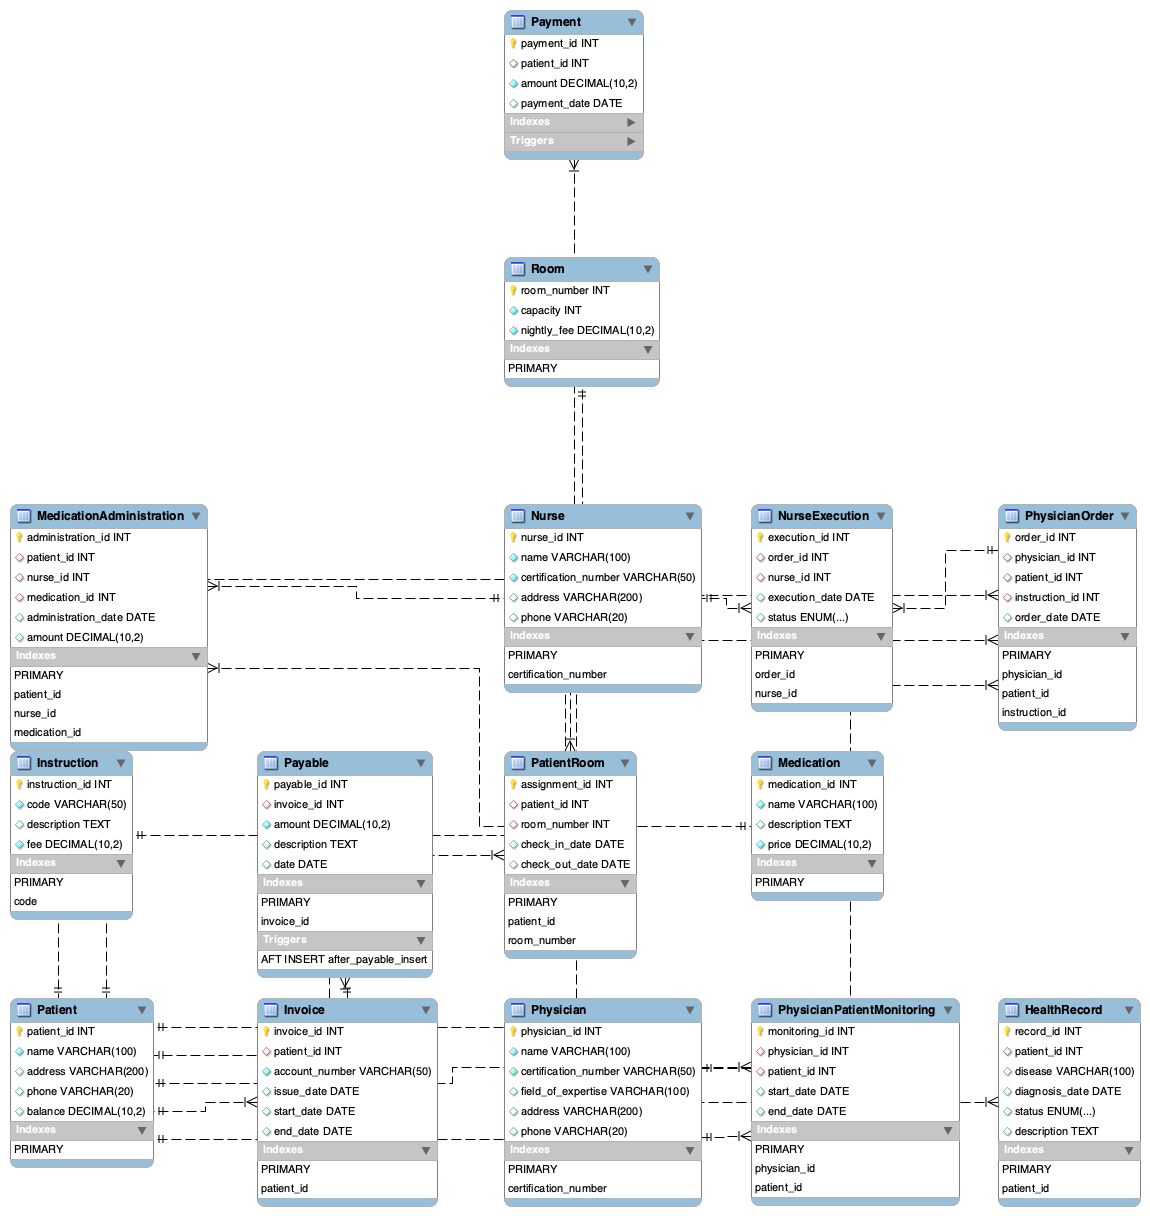
\includegraphics[width=1\textwidth]{hospital.png}
    \caption{Enhanced Entity-Relationship Diagram for the Hospital Database}
\end{figure}

\section{Relations and Keys}
\begin{itemize}
    \item \textbf{Physician(physician\_id, name, certification\_number, field\_of\_expertise, address, phone)}
        \begin{itemize}
            \item Primary Key: \{physician\_id\}
        \end{itemize}
    \item \textbf{Nurse(nurse\_id, name, certification\_number, address, phone)}
        \begin{itemize}
            \item Primary Key: \{nurse\_id\}
        \end{itemize}
    \item \textbf{Room(room\_number, capacity, nightly\_fee)}
        \begin{itemize}
            \item Primary Key: \{room\_number\}
        \end{itemize}
    \item \textbf{Patient(patient\_id, name, address, phone, balance)}
        \begin{itemize}
            \item Primary Key: \{patient\_id\}
        \end{itemize}
    \item \textbf{HealthRecord(record\_id, patient\_id, disease, diagnosis\_date, status, description)}
        \begin{itemize}
            \item Primary Key: \{record\_id\}
            \item Foreign Key: \{patient\_id\} references \textbf{Patient(patient\_id)}
        \end{itemize}
    \item \textbf{PatientRoom(assignment\_id, patient\_id, room\_number, check\_in\_date, check\_out\_date)}
        \begin{itemize}
            \item Primary Key: \{assignment\_id\}
            \item Foreign Keys: \{patient\_id\} references \textbf{Patient(patient\_id)}, \{room\_number\} references \textbf{Room(room\_number)}
        \end{itemize}
    \item \textbf{PhysicianPatientMonitoring(monitoring\_id, physician\_id, patient\_id, start\_date, end\_date)}
        \begin{itemize}
            \item Primary Key: \{monitoring\_id\}
            \item Foreign Keys: \{physician\_id\} references \textbf{Physician(physician\_id)}, \{patient\_id\} references \textbf{Patient(patient\_id)}
        \end{itemize}
    \item \textbf{Medication(medication\_id, name, description, price)}
        \begin{itemize}
            \item Primary Key: \{medication\_id\}
        \end{itemize}
    \item \textbf{MedicationAdministration(administration\_id, patient\_id, nurse\_id, medication\_id, administration\_date, amount)}
        \begin{itemize}
            \item Primary Key: \{administration\_id\}
            \item Foreign Keys: \{patient\_id\} references \textbf{Patient(patient\_id)}, \{nurse\_id\} references \textbf{Nurse(nurse\_id)}, \{medication\_id\} references \textbf{Medication(medication\_id)}
        \end{itemize}
    \item \textbf{Instruction(instruction\_id, code, description, fee)}
        \begin{itemize}
            \item Primary Key: \{instruction\_id\}
        \end{itemize}
    \item \textbf{PhysicianOrder(order\_id, physician\_id, patient\_id, instruction\_id, order\_date)}
        \begin{itemize}
            \item Primary Key: \{order\_id\}
            \item Foreign Keys: \{physician\_id\} references \textbf{Physician(physician\_id)}, \{patient\_id\} references \textbf{Patient(patient\_id)}, \{instruction\_id\} references \textbf{Instruction(instruction\_id)}
        \end{itemize}
    \item \textbf{Payable(payable\_id, invoice\_id, amount, description, date)}
        \begin{itemize}
            \item Primary Key: \{payable\_id\}
            \item Foreign Key: \{invoice\_id\} references \textbf{Invoice(invoice\_id)}
        \end{itemize}
    \item \textbf{Invoice(invoice\_id, patient\_id, account\_number, issue\_date, start\_date, end\_date)}
        \begin{itemize}
            \item Primary Key: \{invoice\_id\}
            \item Foreign Key: \{patient\_id\} references \textbf{Patient(patient\_id)}
        \end{itemize}
    \item \textbf{Payment(payment\_id, patient\_id, amount, payment\_date)}
        \begin{itemize}
            \item Primary Key: \{payment\_id\}
            \item Foreign Key: \{patient\_id\} references \textbf{Patient(patient\_id)}
        \end{itemize}
\end{itemize}

\section{Views and Descriptions}
\subsection{View: Patient Billing}
\lstinputlisting{view-patient-billing.sql}
\textbf{Description}: This view provides a comprehensive billing summary for each patient, including invoice details and total payments made.

\subsection{View: Physician Performance}
\lstinputlisting{view-physician-performance.sql}
\textbf{Description}: This view evaluates physician performance by counting the number of patients monitored and calculating the total revenue generated.

\subsection{View: Room Occupancy Rate}
\lstinputlisting{view-room-occupancy-rate.sql}
\textbf{Description}: This view calculates the occupancy rate for each room, helping to monitor room utilization.

\section{Triggers and Descriptions}
\subsection{Trigger: After Payable Insert}
\lstinputlisting{trig-after-payable.sql}
\textbf{Description}: This trigger updates the patient balance after a new payable is added, ensuring the balance reflects the latest charges.

\subsection{Trigger: After Payment Insert}
\lstinputlisting{trig-after-payment.sql}
\textbf{Description}: This trigger updates the patient balance after a payment is made, ensuring the balance reflects the latest payments.

\subsection{Trigger: Prevent Room Overbooking}
\lstinputlisting{trig-stop-overbooking.sql}
\textbf{Description}: This trigger prevents overbooking of rooms by checking the current occupancy before a new assignment.

\section{Queries, Descriptions, and Results}
\subsection{Query 1: Patient's Medication History}
\lstinputlisting{qr-pt-med-hist.sql}
\textbf{Description}: Retrieves the medication history for each patient, including the patient's name, medication name, administration date, and the nurse who administered the medication.

\subsection{Query 2: Total Medications Administered by Each Nurse}
\lstinputlisting{qr-nurse-meds.sql}
\textbf{Description}: Counts the total number of medications administered by each nurse and orders the results from highest to lowest.

\subsection{Query 3: Patients with Above Average Payments}
\lstinputlisting{qr-pt-ab-avg-payment.sql}
\textbf{Description}: Identifies patients whose total payments are above the average payment amount.

\subsection{Query 4: Physicians with Most Patients}
\lstinputlisting{qr-phys-most-pts.sql}
\textbf{Description}: Finds the physicians who monitor the most patients, sorted by the number of patients in descending order.

\subsection{Query 5: Total Revenue by Medication}
\lstinputlisting{qr-med-rev.sql}
\textbf{Description}: Calculates the total revenue generated by each medication and orders the results by total revenue in descending order.

\subsection{Query 6: Rooms with Above Average Occupancy Rate}
\lstinputlisting{qr-rm-ab-avg-nights.sql}
\textbf{Description}: Identifies rooms that have an occupancy rate above the average occupancy rate.

\subsection{Query 7: Patients and Their Total Expenses}
\lstinputlisting{qr-pt-ttl-expenses.sql}
\textbf{Description}: Retrieves each patient and their total expenses incurred, sorted by the highest total expenses.

\subsection{Query 8: Average Length of Stay per Room}
\lstinputlisting{qr-avg-rm-nights.sql}
\textbf{Description}: Calculates the average length of stay for each room and orders the results from longest to shortest average stay.

\subsection{Query 9: Physicians Treating Most Chronic Cases}
\lstinputlisting{qr-phys-chronic.sql}
\textbf{Description}: Identifies physicians who are treating the most chronic cases (ongoing health records).

\subsection{Query 10: Total Revenue by Physician}
\lstinputlisting{qr-phys-rev.sql}
\textbf{Description}: Calculates the total revenue generated by each physician based on the fees of the instructions they have given.

\subsection{Query 11: Total Number of Treatments per Department}
\lstinputlisting{qr-num-trtmnt-dept.sql}
\textbf{Description}: Finds the total number of treatments ordered per department, sorted by the highest number of treatments.

\subsection{Query 12: Patients with Highest Number of Medications}
\lstinputlisting{qr-pt-high-med.sql}
\textbf{Description}: Retrieves the top 5 patients who have received the highest number of medications.

\subsection{Query 13: Total Revenue by Department}
\lstinputlisting{qr-dept-rev.sql}
\textbf{Description}: Calculates the total revenue generated by each department based on the fees of the treatments they have given.

\subsection{Query 14: Patient Treatment Summary}
\lstinputlisting{qr-pt-treatment-summary.sql}
\textbf{Description}: Provides a summary of the different treatments and medications a patient had been given.


\section{Transactions and Descriptions}
\subsection{Transaction: Patient Admission}
\lstinputlisting{trans-pt-admit.sql}
\textbf{Description}: This transaction inserts a new patient and their initial health record, ensuring atomicity and consistency.

\subsection{Transaction: Patient Discharge}
\lstinputlisting{trans-pt-discharge.sql}
\textbf{Description}: This transaction updates the check-out date for a patient and issues an invoice for the hospitalization period.

\end{document}
% \lstinputlisting{}